\chapter{Rate of return of an Investment}

\section{Discounted Cash Flow Technique}

\begin{definition}
    DCF is a method to measure the \textbf{profitability} of investment projects. Unlike fixed annuities (same payment pattern), DCF allows any pattern of cash inflows (returns) and outflows (costs).
\end{definition}

\begin{comments}
\begin{tabular}{|l|l|l|}
\hline
\textbf{Feature} & \textbf{Annuities} & \textbf{Investments} \\
\hline
Payments & Regular intervals, level payment & May vary in time and amount\\
\hline
Risk & Low/fixed & High/low \\
\hline
Examples & Pensions, loans & Stocks, real estate \\
\hline
\end{tabular}
\end{comments}
\\

\begin{comments}
    There are \textbf{two} DCF measures:
\begin{enumerate}  
    \item Net Present Value (NPV) – Present value of all net cash flows. 
    \item Internal Rate of Return (IRR) – Interest rate that makes NPV = 0. 
\end{enumerate}
\end{comments}







%----------------------------------------
\subsection{Cash flows}

\par Notations with Cash flows:
\begin{itemize}[noitemsep] 
    \item $C_t = \text{contributions/outflows (money invested)}$
    \item $R_t = \text{returns/inflows (money received)}$
    \item $c_t = R_t - C_t = \text{net cash flow at time } t $
\end{itemize}
% $c_t > 0$: Net deposit (inflow)
%     $c_t < 0$: Net withdrawal (outflow)

\begin{comments}
    $c_t > 0$: Net deposit (inflow), 
    $c_t < 0$: Net withdrawal (outflow)
\end{comments}

\begin{example}

\textbf{Project Description:}

A company plans to develop and sell a new product. The cash flows are as follows:

\begin{itemize}
    \item Initial investment of \$80{,}000 at year 0.
    \item Additional investments of \$10{,}000 in years 1, 2, and 3.
    \item A contribution of \$20{,}000 in year 4 to launch the product.
    \item Maintenance costs of \$2{,}000 per year from years 5 to 9.
    \item Returns: \$12{,}000 in year 4, \$30{,}000 in year 5, \$40{,}000 in year 6, \$35{,}000 in year 7, \$25{,}000 in year 8, \$15{,}000 in year 9, and \$8{,}000 in year 10.
\end{itemize}

\textbf{Cash Flow Table:}

\begin{center}
\begin{tabular}{cccc}
\toprule
Year & Contributions & Returns & Net Cash Flow ($c_t$) \\
\midrule
0 & 80{,}000 & 0 & -80{,}000 \\
1 & 10{,}000 & 0 & -10{,}000 \\
2 & 10{,}000 & 0 & -10{,}000 \\
3 & 10{,}000 & 0 & -10{,}000 \\
4 & 20{,}000 & 12{,}000 & -8{,}000 \\
5 & 2{,}000 & 30{,}000 & 28{,}000 \\
6 & 2{,}000 & 40{,}000 & 38{,}000 \\
7 & 2{,}000 & 35{,}000 & 33{,}000 \\
8 & 2{,}000 & 25{,}000 & 23{,}000 \\
9 & 2{,}000 & 15{,}000 & 13{,}000 \\
10 & 0 & 8{,}000 & 8{,}000 \\
\bottomrule
\end{tabular}
\end{center}

\textbf{Net Present Value (NPV):}

Let \( i \) be the interest rate (cost of capital), and let \( v = \frac{1}{1 + i} \). Then the NPV of the project is:

\[
\text{NPV}(i) = \sum_{t=0}^{10} c_t v^t = \sum_{t=0}^{10} \frac{c_t}{(1+i)^t}
\]

Where \( c_t \) is the net cash flow in year \( t \).

\textbf{Interpretation:}
\begin{itemize}
    \item If \( \text{NPV}(i) > 0 \): the investment is profitable.
    \item If \( \text{NPV}(i) = 0 \): the investment breaks even.
    \item If \( \text{NPV}(i) < 0 \): the investment is not worth it.
\end{itemize}
\end{example}






\section{Net Present Value}

\begin{definition}
\textbf{Net present value (NPV)} is the difference between the present value of \textbf{cash inflows} and the present value of \textbf{cash outflows} over a period of time. Choose the investment with the greatest positive NPV.
\end{definition}

\begin{comment}
Goal: Measure whether a project is profitable. 
\end{comment}

\textbf{Formula:}
\[
\text{NPV(i)} = \sum (R_t - C_t) v^t = \sum c_t\cdot v^t
\]


\begin{itemize}
    \item $v^t = \frac{1}{(1+i)^t}$ is the discount factor
    \item $i$ = rate of interest per period = required return of the investment = cost of capital
\end{itemize}

\section{Yield Rate - Internal Rate of Return (IRR)}

\begin{definition}
    \textbf{Yield rate} or IRR is the rate such that the PV of cash inflows is equal to the PV of cash outflows. Choose the investment with the greatest IRR.
\end{definition}

\textbf{Formula:}
\[
\text{IRR} = \text{value of } i \text{ such that } \sum (A_t - L_t) v^t = 0
\]

\textbf{Interpretation:}
\begin{comments}
Yield Rate (IRR) = The interest rate where an investment neither gains nor loses money. 
\begin{itemize}
    \item $\text{NPV} > 0$ : Profit
    \item $\text{NPV} < 0$ : Loss
    \item $\text{NPV} = 0$ : Break-even (Yield rate achieved)
\end{itemize}

Should you still invest when  $\text{NPV} = 0$ ? When  $\text{NPV} = 0$, there is no net gain, but no loss either. Reject the investment if there are better opportunities (i.e. another project with  $\text{NPV} > 0$). Accept it when the Yield rate matched the \textbf{inflation rate}, so your money can keep its real value. 
\end{comments}

\subsection*{Connection Between NPV and IRR}

\begin{itemize}
    \item NPV is a function of the interest rate: $P(i)$
    \item IRR is the rate where $P(i) = 0$
\end{itemize}


\section{Reinvestment}

\subsection{Lump Sum Investment + Interest reinvested}
\begin{definition}
    Intuition: \\
    1. Invest 1 unit of money - \textbf{a lump sum/principal amount} - for n periods at rate $i$. \\
    2. Interest is \textbf{reinvested} at rate $j$. 
\end{definition}

\begin{comments}
    Reinvesting is like planting a tree (investment) and using its seeds (interest) to grow more trees instead of eating them. Over time, you get a forest! 
\end{comments}

\begin{comments}
    Illustration: 
    \begin{enumerate}
        \item Start with 1 unit of money - that principal stays in the account for \textbf{n periods.}
        \item Interest earned per period is 1\$ * $i$ = \$i. The principal gets no compounding effect. 
        \item At the end of year 1,2,...,n-1, we reinvest \$i at each end of the year. This pattern follows an annuity-immediate with \textbf{n payments} of \$i, and rate per period is $j$. 
        \item The \textbf{AV} of that annuity is: i * $s_{\angl{n}j}$. 
        \item Add the principle: Total AV = Principle + Reinvested Interest = 1 + i * $s_{\angl{n}j}$. 
        \end{enumerate}
\end{comments}

\begin{formula} (Lump Sum Reinvestment)
Total Accumulated Value = 1 + i * $s_{\angl{n}j}$
Special case: $i = j$, then AV = $(1+i)^n$
\end{formula}

%-----------------------------------------
\subsection{Annuity + Interest reinvested}
\subsubsection{Annuity-immediate}


\begin{comments}
        \begin{center}
    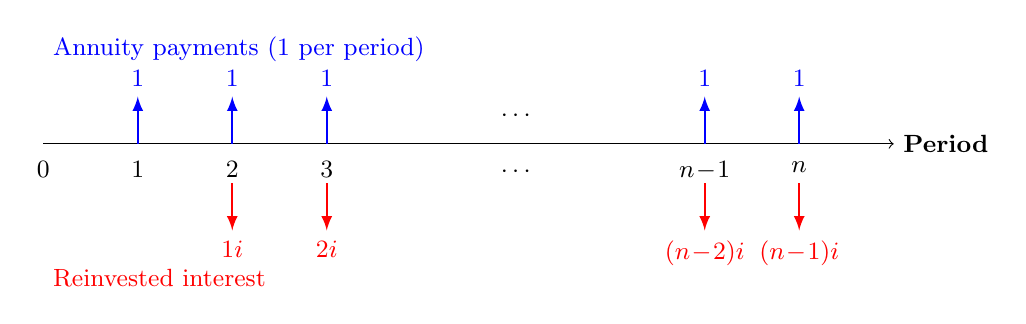
\begin{tikzpicture}[xscale=1.2, font=\small]
    % Timeline
    \draw[->] (0,0) -- (9,0) node[right]{\textbf{Period}};
    
    % Period labels (0 to n)
    \foreach \X in {0,1,2,3} {
        \draw (\X,-0.1) node[below]{$\X$};
    }
    \draw (7,-0.1) node[below]{$n\!-\!1$};
    \draw (8,-0.1) node[below]{$n$};
    
    % Dots for continuation
    \node at (5,0.35) {$\cdots$};
    
    % Annuity payments of 1 at end of each period (starting period 1)
    \foreach \X in {1,2,3} {
        \draw[thick, -latex, blue] (\X,0) -- ++(0,0.6) 
        node[above]{$1$};
    }
    \draw[thick, -latex, blue] (7,0) -- ++(0,0.6) node[above]{$1$};
    \draw[thick, -latex, blue] (8,0) -- ++(0,0.6) node[above]{$1$};
    
    % Reinvested interest labels below timeline (starting period 2)
    \foreach \X [evaluate=\X as \Y using {int(\X-1)}] in {2,3} {
        \draw[thick, -latex, red] (\X,-0.5) -- ++(0,-0.6) 
        node[below]{$\Y i$};
    }
    \draw[thick, -latex, red] (7,-0.5) -- ++(0,-0.6) node[below]{$(n\!-\!2)i$};
    \draw[thick, -latex, red] (8,-0.5) -- ++(0,-0.6) node[below]{$(n\!-\!1)i$};
    
    % Dots for continuation in interest
    \node at (5,-0.35) {$\cdots$};
    
    % Legend
    \node[blue,right] at (0,1.2) {Annuity payments (1 per period)};
    \node[red,right] at (0,-1.7) {Reinvested interest};
    
    % Labels
    % \node[green!70!black] at (0,-0.9) {\textbf{PV}};
    % \node[green!70!black] at (8,-0.9) {\textbf{FV}};
    \end{tikzpicture}
    \end{center}
\end{comments}

\begin{comments}
    AV = sum of annual payments + reinvested interests as annuity \\
    - Reinvested interests as an annuity: i, 2i, 3i, ..., (n-2)i, (n-1)i.
    This acts as an increasing annuity with i as a common difference. \\
    - Sum of annual payments is n. 
\end{comments}

\begin{formula} (Interest Reinvestment as Annuity-immediate)
\[ 
AV = n + i(I_s)_{\angl{n-1}j} = n + i[\frac{s_{\angl{n}j} - n}{j}] \\
\]
\[
AV = s_{\angl{n}i} \text{ when } i = j
\]
\end{formula}

\subsubsection{Annuity-due}
\begin{comments}
        \begin{center}
    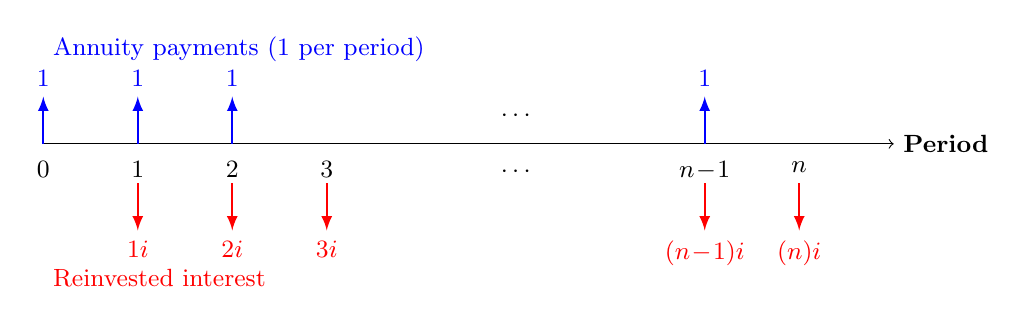
\begin{tikzpicture}[xscale=1.2, font=\small]
    % Timeline
    \draw[->] (0,0) -- (9,0) node[right]{\textbf{Period}};
    
    % Period labels (0 to n)
    \foreach \X in {0,1,2,3} {
        \draw (\X,-0.1) node[below]{$\X$};
    }
    \draw (7,-0.1) node[below]{$n\!-\!1$};
    \draw (8,-0.1) node[below]{$n$};
    
    % Dots for continuation
    \node at (5,0.35) {$\cdots$};
    
    % Annuity payments of 1 at end of each period (starting period 1)
    \foreach \X in {0,1,2} {
        \draw[thick, -latex, blue] (\X,0) -- ++(0,0.6) 
        node[above]{$1$};
    }
    \draw[thick, -latex, blue] (7,0) -- ++(0,0.6) node[above]{$1$};
    
    % Reinvested interest labels below timeline (starting period 2)
    \foreach \X [evaluate=\X as \Y using {int(\X)}] in {1,2, 3} {
        \draw[thick, -latex, red] (\X,-0.5) -- ++(0,-0.6) 
        node[below]{$\Y i$};
    }
    \draw[thick, -latex, red] (7,-0.5) -- ++(0,-0.6) node[below]{$(n\!-\!1)i$};
    \draw[thick, -latex, red] (8,-0.5) -- ++(0,-0.6) node[below]{$(n)i$};
    
    % Dots for continuation in interest
    \node at (5,-0.35) {$\cdots$};
    
    % Legend
    \node[blue,right] at (0,1.2) {Annuity payments (1 per period)};
    \node[red,right] at (0,-1.7) {Reinvested interest};
    
    % Labels
    % \node[green!70!black] at (0,-0.9) {\textbf{PV}};
    % \node[green!70!black] at (8,-0.9) {\textbf{FV}};
    \end{tikzpicture}
    \end{center}
\end{comments}

\begin{formula} (Interest Reinvestment as Annuity-due)
\[ 
AV = n + i(I_s)_{\angl{n}j} = n + i[\frac{s_{\angl{n+1}j} - (n+1)}{j}] \\
\]
\end{formula}

%----------------------------------------
\section{Dollar-weighted Rate of Interest}
\begin{table}[H]
\begin{center}
\renewcommand{\arraystretch}{1.5}
    \begin{tabular}{@{} l l l @{}}
    \toprule
    \textbf{Concept} & \textbf{DWR} & \textbf{IRR (Rate for NPV = 0)} \\
    \midrule
    Purpose & Measures fund performance & Evaluates project profitability \\
    Method & Based on future value & Based on present value \\
    Time orientation & Grows cash to end & Discounts cash to start \\
    Terminology & Used in actuarial \& finance & Used in finance \& investment \\
    \bottomrule
    \end{tabular}

\end{center}
\end{table}

\begin{definition}
    (Dollar-weighted rate of interest) The \textbf{interest rate} $i$ is the average rate of how fast the money grew during a period, based on all the 
    deposits, withdrawals, and interest earned ("dollar-weighted"). 
\end{definition}
\begin{comments}
    Key terms: 
    \begin{itemize}
        \item $A$: Amount at the beginning of the period.
        \item $B$: Amount at the end of the period.
        \item $I$: Total interest earned during the period.
        \item $c_t$: Net contribution (deposit - withdrawal) at time $t\in [0,1]$
        \item $C$ = $\sum{c_t}$: Total net contributions. 
        \item $(1+i)^{1-t}-1$ is the effective rate for period from $t$ to 1. 
    \end{itemize}
\end{comments}

\begin{comments}
    Concept:  \\
    1. Total amount at the end is: $B = A + C + I$ \\
    2. Interest earned: $I = iA + \sum_{0\leq t \leq1}^{} c_t [(1+i)^{1-t} - 1]$
    \par where $iA$ is the interest on initial amount $A$ and $\sum_{0\leq t \leq1}^{} c_t [(1+i)^{1-t} - 1]$
    is the interest on total contributions made at time $t \in [0,1]$. \\
    3. Substitute into 
    \[
    \begin{aligned}
    B &= A + C + I \\
        &= A + C + iA + \sum_{0 \leq t \leq 1} c_t \left[(1+i)^{1-t} - 1\right] \\
        &= A(1+i) + \sum_{0 \leq t \leq 1} c_t (1+i)^{1-t}
        \end{aligned}
        \] 
    4. Approximate the compound interest using simple interest: \\
    \[ {(1+i)}^{1-t} \approx 1 + (1-t)i  \text{ then }
        (1+i)^{1-t} - 1\approx (1-t)i 
    \]
    5. $I = iA + \sum_{0\leq t \leq1}^{} c_t [(1-t)i] = i[A + \sum_{0\leq t \leq1}^{} c_t (1-t)]$ then $i = \frac{I}{A + \sum_{0\leq t \leq1}^{} c_t (1-t)}$\\
\end{comments}

\begin{formula}
    \[ i \approx \frac{I}{A + \sum_{0\leq t \leq1}^{} c_t (1-t)} = \frac{\text{Interest earned}}{\text{Exposure}}\]
    The approximation is good when each contribution $c_t$ is small compared to the amount $A$. 
\end{formula}

\begin{comments}
    The denominator is called \textbf{exposure associated with }$i$ \& represents \textbf{total time-weighted amount of money at risk}: 
    \begin{itemize}
        \item $A$: Initial fund amount that earns interest for the full year - its weight = 1. 
        \item $\sum_{0\leq t \leq1}^{} c_t (1-t)$: time-weighted contributions, giving how long each contribution had to earn interest 
            ($c_t$ it the contribution made at time $t$ and $(1-t)$= weight is the fraction of the year left in which the contribution
        earns interests.)
    \end{itemize}
\end{comments}

\begin{formula}
    (Exposure)
    \[ A + \sum_{0\leq t \leq1}^{} c_t (1-t) \]
    Exposure is as a weighted sum of how much money was active in the fund and for how long. 
\end{formula}

\begin{example}
    At the beginning of a year, an investment fund was established with an initial deposit of \$3,000.
    At the end of six months, a new deposit of \$1,500 was made. Withdrawals of \$500 and \$800 were
    made at the end of four months and eight months respectively. The amount in the fund at the end
    of the year is \$3,876. Set up the equation of value to calculate the dollar-weighted rate of interest. 
    \newline
    \begin{solution}
        To find the interest rate $i$ that makes the future value of all cash flows = \$3876. 

        General formula: 
        \[
            \text{Future Value} = \sum c_t (1+i)^{1-t}
        \]

        Set up the equation of value to calculate the dollar-weighted rate of interest $i$:

        \[
        3000(1 + i) 
        + 1500(1 + i)^{0.5} 
        - 500(1 + i)^{(1 - \frac{4}{12})}
        - 800(1 + i)^{(1 - \frac{8}{12})} 
        = 3876
        \]
    \end{solution}
\end{example}


\section{Time-weighted Rate of Interest}
\begin{definition}
    \textbf{Time-weighted rate of return} isolates fund performance and ignores investor actions. 
    \[ i = (1+j_1)(1+j_2)...(1+j_m) - 1 \]
    where $j_k$ is the rate of return for each sub-period in an interval (in this case, a year) which has m sub-periods.
\end{definition}

\begin{comments}
    \textbf{Set up: } \\
    \begin{itemize}
        \item The year is split into m intervals (sub-periods)
        \item At each time $t_k$, 
            \subitem  $C_{t_k}$ = net contribution
            \subitem  $B_{t_k}$ = fund value just before that contribution
    \end{itemize}

    then for each subinterva; $k = 1,2,...,m$, the rate of return $j_k$ for each sub-period is
    \[ B_{t_k} = (1+j_k)(B_{t_{k-1}} + C_{t_{k-1}}) \]
    The overall yield rate $i$ for the entire year is given by
    \[ i + 1 = (1+j_1)(1+j_2)...(1+j_m) \]
    We call $i$ the \textbf{time-weighted rate of return.}

\end{comments}